% Modello di presentazione di tesi al computer.
% Collaudato sia con LaTeX che con pdfLaTeX.
% Richide alcuni file di stile
% (marslide.sty marsdefs.sty mars-cds.sty hugefonts.sty)
% e alcune figure, che sono forniti insieme
% con questo file.
% Scritto da Gianluca Gorni
% Versione: 9 novembre 2006

\documentclass[italian,landscape]{report}

\usepackage[italian]{babel}
\usepackage[utf8]{inputenc}
\usepackage{uniudpres}

\graphicspath{{./img/}}

\usepackage{impostazionipresentazione}
\begin{document}

\maketitle

\tableofcontents
% Provare come viene l'indice a doppia colonna:
% \indicedoppiacolonna

\chapter{Alcune cose\label{intestazioneCapitolo}}

%%%%%%%%%%%%%%%%%%%%%%%%%%%%%%%%%%%%%%%%%

\section{Capitoli e sezioni}

\begin{firstheadlineitemize}
\item La schermata di apertura \`e un'\rosso{intesta\-zione generale} per tutto il documento.
\pause
\item I \rosso{capitoli} (facoltativi) hanno un'intestazione a tutta pagina.
\pause
\item Le \rosso{sezioni} hanno il titolo nella fascia blu in cima.

\begin{secondheadlineitemize}
\pause
\item Le sezioni non sono numerate.

%%%%%%%%%%%%%%%%%%
\newpage
\item Il titolo in alto rimane su tutte le schermate fino alla fine della sezione.
\end{secondheadlineitemize}
\end{firstheadlineitemize}

%%%%%%%%%%%%%%%%%%%
\section{A tutto schermo}
\begin{firstheadlineitemize}
\item Il documento \`e pensato per essere proiettato \rosso{a tutto schermo}
\pause
\begin{secondheadlineitemize}
\item Quando a tutto schermo, si possono avanzare o retrocedere le pagine in vari modi:
\begin{thirdheadlineitemize}
\pause
item premendo le frecce della tastiera;
\pause
\item cliccando sui triangoli \indietro{} \avanti{} in alto a destra;
\pause
\item cliccando in un punto generico dello schermo col tasto sinistro o destro del mouse.
\end{thirdheadlineitemize}
\pause
\item Per tornare da schermo pieno a finestra normale, un modo \`e di premere il tasto \sfondogiallo{\rosso{\texttt{esc}}}.
\end{secondheadlineitemize}
\end{firstheadlineitemize}

%%%%%%%%%%%%%%%%%%%%%%%%%%%%%%%%%%%%%%%%%%%%%%%%%%%%%%%%%
\section{Punti e pause}
\begin{firstheadlineitemize}
\item Primo livello
\pause
\item Ancora primo livello
\pause
\begin{secondheadlineitemize}
\item Secondo livello
\pause
\item Ancora secondo livello
\end{secondheadlineitemize}
\pause
\item Notare le pause!
\pause
\begin{secondheadlineitemize}
\item Prima aggiunta, al secondo livello.
\pause
\begin{thirdheadlineitemize}
\item Aggiunta al terzo livello
\pause
\begin{fourthheadlineitemize}
\item S\`{\i}, c'\`{e} anche il quarto.
\pause
\end{fourthheadlineitemize}
\end{thirdheadlineitemize}
\end{secondheadlineitemize}
\item Non spezzate una frase fra due pagine!
\pause
\begin{secondheadlineitemize}
\item Usare \rosso{\texttt{\symbol{92}section}} o \rosso{\texttt{\symbol{92}newpage}}
\end{secondheadlineitemize}
\end{firstheadlineitemize}

%%%%%%%%%%%%%%%%%%%%%%%%%%%%%%%%%%%%%%%%%%%%%%%%%%%%%%%%%%%%

\section{Dimensioni e colori}

\begin{firstheadlineitemize}

\item \small Piccolo. \large Medio. \Large Grande. \huge Grandissimo.

\pause
\bigskip

\item \textcolor{red}{Rosso.} \textcolor{green}{Verde.} \verdescuro{Verde scuro.} \ocra{Ocra.}

\end{firstheadlineitemize}

\pause

\bigskip

\begin{thirdheadlineitemize}

\item Per un elenco di dimensioni e colori predefiniti vedere la documentazione \textcolor{darkorange}{\texttt{marslides-doc.pdf}} reperibile presso

\end{thirdheadlineitemize}

\begin{center}
\url{http://www.cds.caltech.edu/~wgm/WARM/slides/marslide/}
\end{center}

%%%%%%%%%%%%%%%%%%%%%%%%%%%%%%%%%%%%%%%%%%%%%%%%%%%%%%%%
\section{Formule}


\begin{secondheadlineitemize}

\item Formula:
$$\int_0^1x^2\,dx$$

\pause

\item Formula centrata orizzontalmente nella pagina, con sfondo giallo:
\displaysfondogiallo{\int_0^1x^2\,dx}

\pause

\item Formula che appare un poco per volta:

\pause

\parstepwise{
$$
  1\step{{}+2}
  \step{{}+3} \step{{}+4}\step{{}+\cdots+n}
  \step{{}={}}
  \step{\sfondogiallo{$\displaystyle\frac{n(n+1)}{2}$}}
$$
}

\end{secondheadlineitemize}

%%%%%%%%%%%%%%%%%%%%%%%%%%%%%%%%%%%%%%%%%%%%%%%%%%%%%%%%

\chapter{Altre cose}

%%%%%%%%%%%%%%%%%%%%%%%%%%%%%%%%%%%%%%%%%%%%%%%%%%%

\section{Enunciati e figure}

\begin{firstheadlineitemize}

\item[] \textbf{Teorema di Pitagora.}
\rosso{La somma dei quadrati costruiti sui cateti \`{e} uguale al quadrato costruito sull'ipotenusa.}

\end{firstheadlineitemize}

\pageTransitionGlitter{0}

\pause

\begin{center}
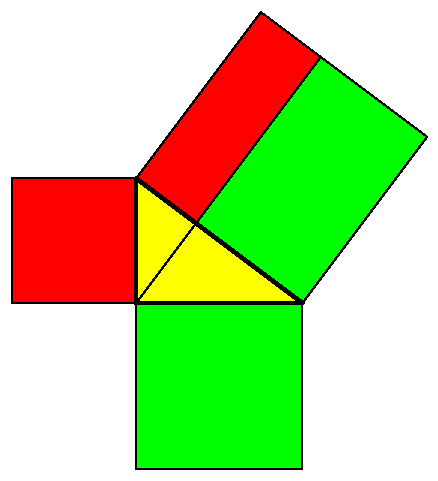
\includegraphics[scale=1.5]{pitagora3}
\end{center}

%%%%%%%%%%%%%%%%%%%%%%%%%%%%%%%%%

\section{Figure progressive}

\begin{center}
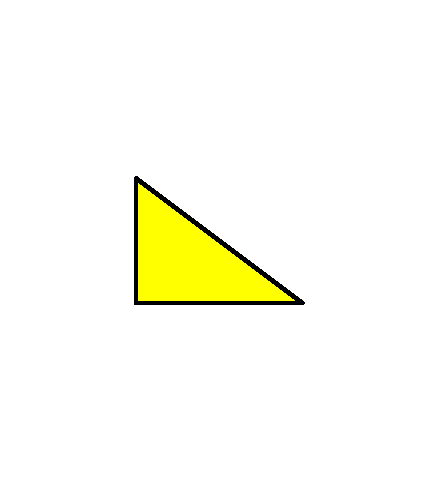
\includegraphics[scale=1.2]{pitagora1}
\end{center}

\begin{firstheadlineitemize}

\item \textbf{Teorema di Pitagora:}

\pause

\begin{secondheadlineitemize}

\item In un triangolo rettangolo

\end{secondheadlineitemize}

\end{firstheadlineitemize}

% il comando \newframe e' come \newpage,
% ma non avanza il numero di pagina.
% Puo' servire per fare cambiamenti incrementali
% a una pagina, quando \pause o \stepwise non
% bastano. In questo esempio \pause non va bene
% perche' qui bisogna aggiungere un paragrafo
% ma allo stesso tempo  cambiare la figura che
% sta in cima alla pagina. Macchinoso da scrivere,
% ma puo' valerne la pena.
%%%
\newframe


\begin{center}
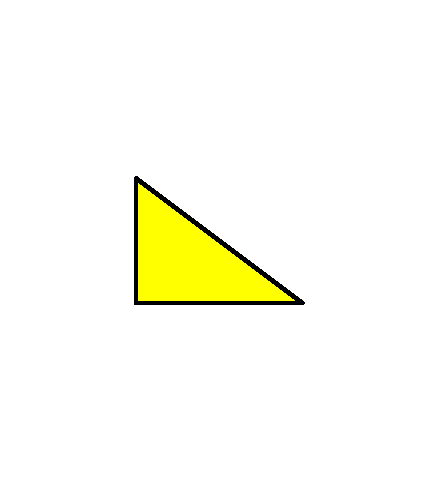
\includegraphics[scale=1.2]{pitagora1}
\end{center}

\begin{firstheadlineitemize}

\item \textbf{Teorema di Pitagora:}

\begin{secondheadlineitemize}

\item  In un triangolo rettangolo \sfondogiallo{\rosso{\textit{coincidono:}}}

\end{secondheadlineitemize}

\end{firstheadlineitemize}

%%%%
\newframe

\begin{center}
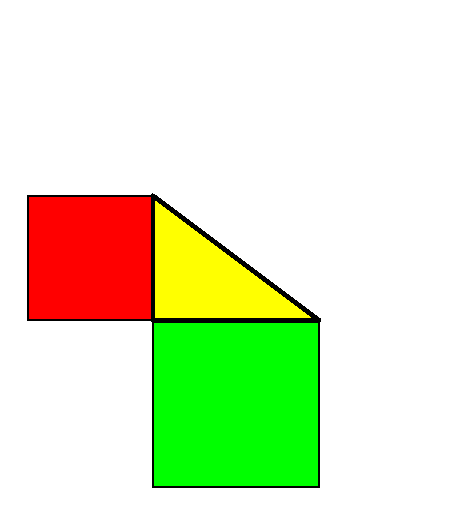
\includegraphics[scale=1.2]{pitagora2}
\end{center}

\begin{firstheadlineitemize}

\item \textbf{Teorema di Pitagora:}

\begin{secondheadlineitemize}

\item  In un triangolo rettangolo \sfondogiallo{\rosso{\textit{coincidono:}}}

\begin{thirdheadlineitemize}

\item la somma dei quadrati costruiti sui cateti

\end{thirdheadlineitemize}

\end{secondheadlineitemize}

\end{firstheadlineitemize}

%%%
\newframe

\begin{center}
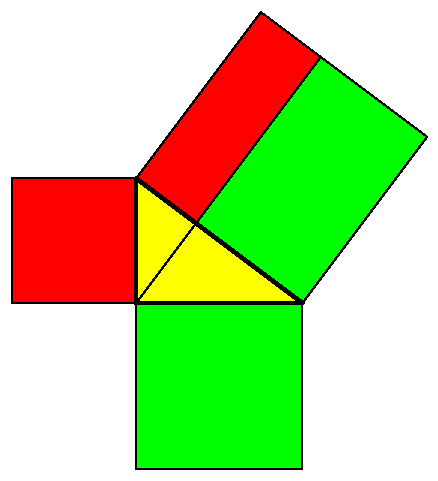
\includegraphics[scale=1.2]{pitagora3}
\end{center}

\begin{firstheadlineitemize}

\item \textbf{Teorema di Pitagora:}

\begin{secondheadlineitemize}

\item  In un triangolo rettangolo \sfondogiallo{\rosso{\textit{coincidono:}}}

\begin{thirdheadlineitemize}

\item la somma dei quadrati costruiti sui cateti

\item e il quadrato costruito sull'ipotenusa.

\end{thirdheadlineitemize}

\end{secondheadlineitemize}

\end{firstheadlineitemize}

\pageTransitionBlindsV

%%%%%%%%%%%%%%%%%%%%%%%%%%%%%%%%%%%%%%%%%%%%%%%%%%%%%%%%

\section{Transizioni}

\pageTransitionWipe{0}

\begin{firstheadlineitemize}

\item Visto che transizioni pdf?

\pause

\begin{secondheadlineitemize}

\item Belle, eh?

\end{secondheadlineitemize}

\pause

\pageTransitionWipe{180}

\item E ce ne sono tante altre!

\pause

\begin{secondheadlineitemize}

\pageTransitionSplitVO

\item {\setlength{\baselineskip}{2\baselineskip}
Vedere la documentazione del pacchetto \textcolor{darkorange}{\texttt{texpower}}.
}

\end{secondheadlineitemize}

\end{firstheadlineitemize}

\pause

\begin{center}
\url{http://texpower.sourceforge.net/}
\end{center}

\pageTransitionReplace

%%%%%%%%%%%%%%%%%%%%%%%%%%%%%%%%%%%%%%%%%%%%%%%%%%%%%%%%%%
\section{Altro}

\begin{secondheadlineitemize}

\item[] Una formula che compare da dentro a fuori:

\pause

 \parstepwise
  {$$\step[\value{step}=2]{f^{-1}\bigl(}
    \step[\value{step}=1]{f(}
    \textcolor{red}{x}
    \step[\value{step}=1]{)}
    \step[\value{step}=2]{\bigr)}
    \step[\value{step}=3]{=\textcolor{red}{x}.}$$
    }

\end{secondheadlineitemize}


\pageTransitionBoxI

\end{document}